\documentclass[dvisvgm,tikz]{standalone}
\usepackage{circuitikz}
\usepackage{tabularray}
\renewcommand{\familydefault}{\sfdefault}
\begin{document}
\definecolor{gold}{rgb}{0.83, 0.69, 0.22}
\definecolor{silver}{rgb}{0.75, 0.75, 0.75}
\newcommand\Stripe[2]{\draw[fill=#2,#2] ++(#1,0) +(-0.15,-0.71) rectangle +(0.15,0.71);}
\newcommand\stripe[2]{\draw[fill=#2,#2] ++(#1,0) +(-0.15,-0.51) rectangle +(0.15,0.51);}
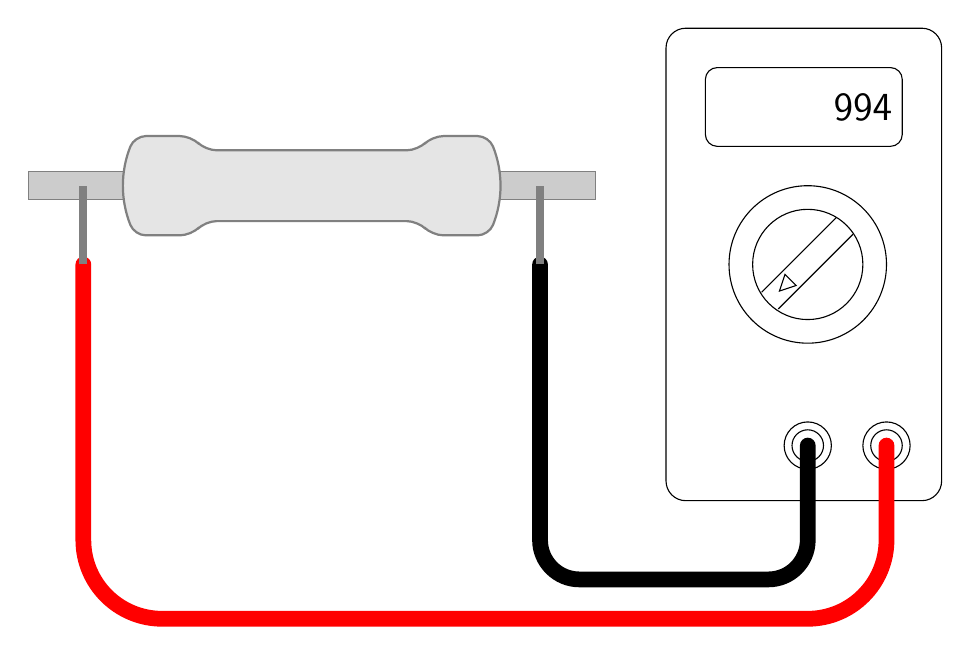
\begin{tikzpicture}
  \begin{scope}[shift={(3.5,6)},scale=0.9]
    % wire
    \draw[gray,fill=gray!40] (-4,-0.2) rectangle (4,0.2);
    % resistor
    \draw[rounded corners,thick,gray,fill=gray!20]
    ++(0,0.5) -- ++(1.5,0) -- ++(0.2,0.2) -- ++(0.8,0)
    .. controls +(0.2,-0.5) and +(0.2,0.5) .. ++(0,-1.4) -- ++(-0.8,0)
    -- ++(-0.2,0.2) -- ++(-3,0) -- ++(-0.2,-0.2) -- ++(-0.8,0)
    .. controls +(-0.2,0.5) and +(-0.2,-0.5) .. ++(0,1.4) -- ++(0.8,0)
    -- ++(0.2,-0.2) -- cycle;
    % band colors
    \stripe{-1.0}{brown}
    \stripe{0.0}{black}
    \stripe{1.0}{red}
    \Stripe{2.1}{gold!100!gray}
  \end{scope}

  % multimeter
  \draw[rounded corners=0.25cm] (11.5,2) rectangle (8,8);
  \draw[rounded corners=0.15cm] (11,6.5) rectangle (8.5,7.5);
  \node at (10.5,7) {\Large 994};
  \draw (9.8,5) circle (1);
  \draw (9.8,5) circle (0.7);
  \begin{scope}[shift={(6.40,-5.45)}, rotate=45]
    \draw (9.13,5.15) -- (10.47,5.15);
    \draw (9.13,4.85) -- (10.47,4.85);
    \draw (9.3,5) -- (9.5,5.1) -- (9.5,4.9) -- cycle;
  \end{scope}
  \node at (8.8,4) {\Large\si{\ohm}};
  \draw (9.8,2.7) circle (0.3);
  \draw (9.8,2.7) circle (0.2);
  \draw (10.8,2.7) circle (0.3);
  \draw (10.8,2.7) circle (0.2);
  
  % test lead set
  \draw[line width=2mm, color=red, line cap=round, rounded corners=1cm] (10.8,2.7) -- (10.8,0.5)
  -- (0.6, 0.5) -- (0.6,5);
  \draw[line width=2mm, color=black, line cap=round, rounded corners=5mm] (9.8,2.7) -- (9.8,1)
  -- (6.4, 1) -- (6.4,5);
  \draw[line width=1mm, color=gray] (0.6,5) -- (0.6,6);
  \draw[line width=1mm, color=gray] (6.4,5) -- (6.4,6);
\end{tikzpicture}
\end{document}